\chapter{Problemi e complessità}

\section{Problemi}

\subsection{Definizione formale}
Prima di definire cosa siano gli \textit{algoritmi}, è necessario definire
formalmente cosa sia un \textit{problema}; un problema $\Pi$ è definito da:
\begin{itemize}
	\setlength\itemsep{0pt}
	\item l'insieme degli input del problema $I_{\Pi}$;
	\item l'insieme degli output del problema $O_{\Pi}$; e
	\item una funzione $Sol_{\Pi}: I_{\Pi} \rightarrow \{2^{O_{\Pi}} \setminus \emptyset\}$,
	      interpretata come una funzione che associa ad ogni input i relativi
	      output corretti per il problema - in altre parole, la funzione calcola
	      un sottoinsieme non vuoto di $O_{\Pi}$ che risolve il problema per il dato input\footnote{
		      La funzione ha come codominio un insieme di funzioni, di conseguenza
		      si può vedere come una curryficazione di $Sol: I \times O \rightarrow 2$, che indica se,
		      effettivamente, un output sia valido un certo input.}.

\end{itemize}

\subsubsection{Esempi}
\paragraph{1}
\prob {NPrime} {$\mathbb{N}$} {$\{0, 1\} = 2$} {$n \in \mathbb{N}$ è primo?}

è un problema di \textbf{decisione}.

\paragraph{2}
\prob {MCD} {$\mathbb{N}\times\mathbb{N}$} {$\mathbb{N}$}
{Trova il massimo comun divisore tra due numeri.}

\paragraph{3}
\prob {SAT} {CNF ben formate} {$\{0, 1\} = 2$} {\`E possibile soddisfare la formula in input?}

è nuovamente un problema di decisione.

\section{Rappresentazioni}
% @TODO: Riguardare questa lezione, la spiegazione qui sotto non è 
% affatto chiara. 
In modo da poter definire formalmente gli algoritmi prendendo come modello
di riferimento le macchine di Turing, assumiamo

$$
	I_{\Pi} \subseteq 2^2
$$
e
$$
	O_{\Pi} \subseteq 2^2
$$
Assumiamo di dover scrivere in binario i due numeri $3$ e $5$, ossia $11$ e $101$.
Per dare i due input ``in pasto'' alla macchina di Turing non possiamo
semplicemente concatenare le due stringhe: $11101$ sarebbe un altro numero
($29$, in particolare). Possiamo utilizzare un trucco, ossia raddoppiamo ogni
bit: $1111$, $110011$. Si nota facilmente che non compare mai la coppia $01$ o
$10$ leggendo i bit due a due; si potranno utilizzare quindi questi marker per
segnalare la fine di un numero e l'inizio di un altro.

Avremo spesso a che fare con input più complicati
(si pensi al \textsc{TSP}: matrici di incidenza, liste di adiacenza, ...);
se ci sono molti modi diversi per \textbf{codificare} l'input, parlare informalmente
dei problemi causa problemi nel definire (e implementare, ovviamente)
gli algoritmi, addirittura arrivando a cambiare la complessità dell'algoritmo
in base alla codifica utilizzata.

Per il livello di dettaglio al quale noi vogliamo scendere nello studio della
complessità, sarà sufficiente non dare molto peso in termini di differenza di complessità
alle rappresentazioni, introducendo una leggera imprecisione. In termini pratici,
come \textit{regola del pollice}, si può notare che la distanza indotta,
in termini di complessità, dal cambio di rappresentazione è polinomialmente
limitata: si prenda l'esempio della rappresentazione a matrici di incidenza
per i grafi sparsi; nonostante essi siano \textit{meno efficienti} delle liste
di adiacenza, ci si accorge facilmente che la distanza è limitata polinomialmente.

Tuttavia, non è sempre questo il caso: si prenda per esempio la rappresentazione
binaria di un numero, e.g. \texttt{10100}, e la sua rappresentazione unaria
\texttt{000000000000000000001}. \`E chiaro che il rapporto tra le due
rappresentazioni non sia polinomiale: il confine tra polinomiale e ``probabilmente
non polinomiale'' contiene dei problemi che hanno una complessità esponenziale
se l'input è in rappresentazione binaria e ``diventano'' polinomiali se l'input
è unario.

Gonfiando artificialmente l'input, il costo in tempo dell'algoritmo - che è
rappresentato in termini della lunghezza dell'input - necessariamente decresce.
In questo senso, se l'algoritmo è polinomiale nel \textit{valore} dell'input
ma non necessariamente nella sua lunghezza, esso è detto \textbf{pseudo-polinomiale}.

\section {Algoritmi}
Un algoritmo $A$ per un problema $\Pi$ è una funzione
$$
	A: I_{\Pi} \rightarrow O_{\Pi}
$$
O, localmente,
$$
	x \mapsto y
$$
tale che  $y \in Sol_{\Pi}(x)$ (o, alternativamente, $Sol_{\Pi}(x)(y) = 1$),
ossia una soluzione \textit{corretta} per $x$.

In termini formali, un algoritmo rappresenta una \textit{macchina di Turing}.
Tuttavia, non scenderemo mai ad un livello di dettaglio tale per cui dovremo descrivere,
effettivamente, un programma in termini di MdT, che richiederebbe uno sforzo
non indifferente; utilizzeremo invece una notazione relativamente informale
basata sullo \textit{pseudocodice}.

Ciò che ci interessa degli algoritmi è studiare la loro \textbf{complessità}.
Quando si parla di complessità, si possono adottare due accezioni:
complessità \textbf{algoritmica} e complessità \textbf{strutturale}.

\subsection{Complessità algoritmica}
Chiedersi se un determinato problema $\Pi$ può essere risolto
non è banale, affatto (basta seguire un qualsiasi corso di informatica teorica
per rendersene conto) - e anche per una semplice argomentazione di cardinalità\footnote{
	Tra tanti, due testi che trattano la calcolabilità sono \cite{Hopcroft:79:introLFA} e
	\cite{Kfoury:82:programcomput}.
}
ci possiamo rendere conto che esiste una quantità più che numerabile di problemi
che può essere risolta da un numero numerabile di algoritmi. La teoria della
calcolabilità è l'area che si occupa di questi problemi.

Per quanto riguarda il nostro corso, ci terremo dall'altra parte della barricata,
ossia tratteremo solo problemi che sappiamo essere calcolabili, ossia problemi
$\Pi$ per i quali esiste un algoritmo $A$ che lo risolve.
Ma non tutti gli algoritmi sono equivalenti: ci interessa
infatti studiare ``quanto costa'' un algoritmo, e dovremo di conseguenza
adottare una misura di costo (spazio sul nastro, istruzioni eseguite,...)

\subsubsection{Costo}
Definiamo quindi una funzione di costo:
$$
	T_A : I_{\Pi} \rightarrow \mathbb{N}
$$
che dipende da ciò che vogliamo calcolare; così com'è, però, è difficile da
utilizzare con l'obiettivo di confrontare due algoritmi. \`E preferibile
lavorare per ``taglia'', ossia per dimensione dell'input;
definiamo quindi una funzione
$$
	t_A:\mathbb{N} \rightarrow \mathbb{N} ~~~ \text{dove} ~~~ t_A(n) = max\{T_A(x)|x \in I_{\Pi} \land |x| = n\}
$$
che è chiamata \textit{semplificazione del caso peggiore}; chiaramente, si ha
che $t_A$ è una valutazione pessimista del costo: per esempio, se $t_A(100) = 7500$
significa che su input di grandezza $100$ il costo \textit{massimo} è $7500$.
La complessità \textbf{algoritmica} utilizza proprio queste funzioni
per confrontare due algoritmi. Dati $A_1$ e $A_2$ possiamo disegnare $t_{A_1}$
e $t_{A_2}$ come in figura \ref{fig:t1t2algcomp}.


\begin{figure}[ht]
	\centering
	\begin{tikzpicture}
		\begin{axis}[
				axis lines = middle,
				xlabel = {$n$},
				ylabel = {$T$},
				yticklabels={,,},
				xticklabels={,,}
			]

			\addplot [name path = A,
				-,
				domain = 0:4.5,
				samples = 1000] {x^2}
			node [near end, right] {$t_{A_1}$};

			\addplot [name path = B,
				-,
				domain = 0:4.5] {x^(1/2)}
			node [very near end, above] {$t_{A_2}$};

		\end{axis}
	\end{tikzpicture}
	\caption{Complessità algoritmica semplificata nel caso peggiore per due funzioni $t_{A_1}$ e $t_{A_2}$.}
	\label{fig:t1t2algcomp}
\end{figure}

A questo punto, possiamo interessarci alle fasce di grandezza e capire, in un
certo range, quale algoritmo scegliere, oppure fare un'assunzione asintotica
scegliendo l'algoritmo che asintoticamente cresce di meno.

\paragraph{Upper e lower bound, ottimalità}
Supponiamo di aver trovato un algoritmo $A$ la cui complessità è $O(n^{2.37})$.
Questo valore è un \textit{upper bound}. Siamo sicuri di non poter fare di meglio?
Raramente si è certi: qui interviene un tipo di ragionamento completamente
diverso, il cui obiettivo è dimostrare che più di tanto per un certo problema
non si può fare, dimostrando quindi dei \textit{lower bound}. In questo contesto
si cercano dimostrazioni, non algoritmi. Trovando, per esempio, che il lower
bound teorico per il problema è $\Omega(n^2)$, non si sanulla del range tra
$n^2$ e $n^{2.37}$ e, idealmente, si continuerà a cercare un algoritmo finché si arriva ad un
algoritmo $O(n^2)$, che è (asintoticamente) ottimale. Pochissimi problemi
godono di un algoritmo ottimale: uno dei pochi è l'ordinamento di array, che ha
complessità ottimale $\Theta(n\cdot log(n))$. Tuttavia, questo non significa
che \textit{heapsort}, per esempio, sia l'algoritmo \textit{migliore} in toto:
la pratica spesso smentisce queste possibilità. Un esempio è l'algoritmo
di Danzig, in teoria esponenziale e in pratica migliore di altri algoritmi
polinomiali.

\subsection{Complessità strutturale}
L'obiettivo finale della complessità algoritmica è trovare un algoritmo
ottimo per ogni problema. Questo obiettivo è, chiaramente, quasi sempre
irraggiungibile. Immaginiamo, per un momento, di conoscere tutte le complessità
ottimali dei problemi: la complessità strutturale parte dal presupposto che
per ogni problema si possa definire la \textit{sua} complessità, in modo da
poter collocare ogni problema in una precisa \textbf{classe}.

\subsubsection{Classi di complessità}
Solitamente, la complessità strutturale si occupa esclusivamente di problemi 
di decisione, i quali sono analoghi al problema dell'appartenenza di una 
\textit{parola} ad un \textit{linguaggio}; pertanto tutti i problemi di decisione 
sono dei sottoinsiemi di $2^{2^*}$ e un sottoinsieme in particolare è 
l'insieme di \textit{tutti i problemi decidibili in tempo polinomiale} $\mathbf{P}$. 

Per molti problemi vorremmo sapere se esso appartiene o meno a 
$\mathbf{P}$ ma, al momento, non abbiamo modo di saperlo: 
un esempio è SAT. Allo scopo di arrivare ad una risposta a questa domanda, 
è stato ``inventata'' la classe di complessità $\mathbf{NP}$\footnote{Per approfondire queste 
tematiche consultare \cite{Arora:09:computcompl} e \cite{complexityzoo}.}.

\begin{figure}[ht]
	\centering
	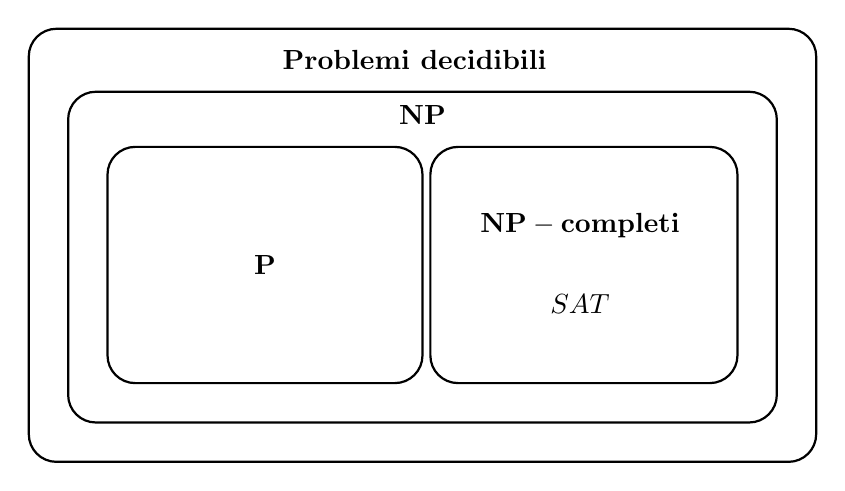
\begin{tikzpicture}[scale=1.0]
		\draw[black,rounded corners=10,thick]
		(0,0) rectangle (10,5.5);
		\draw[black,rounded corners=10,thick]
		(4.9,5.1) node {\bf Problemi decidibili};

		\draw[black,rounded corners=10,thick]
		(0.5, 0.5) rectangle (9.5,4.7);
		\draw[black,rounded corners=10,thick]
		(5,4.4) node {$\mathbf{\mathbf{NP}}$};

		\draw[black,rounded corners=10,thick]
		(1,1) rectangle (5,4);
		\draw[black,rounded corners=10,thick]
		(3,2.5) node {$\mathbf{\mathbf{P}}$};

		\draw[black,rounded corners=10,thick]
		(5.1,1) rectangle (9,4);
		\draw[black,rounded corners=10,thick]
		(7,3) node {\bf $\mathbf{NP-completi}$};
		\draw[black,rounded corners=10,thick]
		(7,2) node {$SAT$};

	\end{tikzpicture}
	\caption{Classi di complessità strutturale.}
	\label{fig:structcomplclass}
\end{figure}

\subsubsection{Riducibilità}
Il concetto di \textbf{riducibilità} (in tempo polinomiale) gioca una parte
fondamentale nella teoria della complessità strutturale: si dice che un problema $\Pi_1$
è polinomialmente riducibile ad un problema $\Pi_2$ se e solo se
$$
	\exists f: 2^* \rightarrow 2^*
$$
tale che:
\begin{itemize}
    \setlength\itemsep{0pt}
	\item $f$ è calcolabile polinomialmente
	\item $\forall x \in I_{\Pi_1}  ~~ f(x) \in I_{\Pi_2}$
	\item $\forall x ~~ Sol_{\Pi_2}(x) = 1 \iff Sol_{\Pi_1}(x) = 1$
\end{itemize}

Questa definizione ha come conseguenza il seguente lemma.
\begin{lemma}\label{lem:poli_red}
	Se $\Pi_2 \in \mathbf{P}$ e $ \Pi_1 \leq_{p} \Pi_2$,
	ossia $\Pi_1$ è riducibile polinomialmente a $\Pi_2$, allora $\Pi_1 \in \mathbf{P}$.
\end{lemma}
La classe dei problemi $\mathbf{NP-completi}$ è quindi definita come
$$
	\mathbf{NP-completi} = \{\Pi \in \mathbf{NP} | \forall \Pi'\in \mathbf{NP} ~~ \Pi' \leq_{p} \Pi\}
$$
\begin{theorem}[di Cook]
	$SAT \in \mathbf{NP-completi}$.
\end{theorem}
\chapter{Problemi di ottimizzazione}
\section {Introduzione}
Un problema di \textbf{ottimizzazione} è caratterizzato da: 
\begin{enumerate}
  \item  è l'insieme degli input $I_{\Pi}$;
  \item  è l'insieme degli output $O_{\Pi}$;
  \item  una funzione che ad ogni input associa una famiglia di output: $Amm_{\Pi} : I_{\Pi} \rightarrow \{2^{O_{\Pi}} \setminus \emptyset \}$;
  \item il tipo del problema $Tipo_{\Pi} \in \{Min, Max\}$; e
  \item una funzione da una coppia input-output ai naturali
    $$
	c_{\Pi}: I_{\Pi}\times O_{\Pi} \rightarrow \mathbb{N}
    $$
    che formalizza il concetto di \textbf{costo} di una soluzione - per un problema 
    di minizzazione, l'obiettivo sarà scegliere l'output con costo minore. 

\end{enumerate}
Le proprietà $3$, $4$ e $5$ formalizzano ulteriormente l'insieme $Sol_{\Pi}$ definito in precedenza. 
\subsection{Esempi}
\subsubsection{MaxSat}

\popt{MaxSAT}
{CNF ben formate}
{$\mathbb{N}$} 
{Qual è il numero massimo di clausole che si possono verificare?} 
{Assegnamenti di valori di verità coerenti} 
{$Max$}
{Numero di clausole rese vere}

\noindent
Le istanze di questo problema sone formule in forma normale congiunta ben formate
(ossia CNF); le soluzioni ammissibili sono assegnamenti di valori di verità; 
il costo (o \textit{funzione obiettivo}) è il numero di clausole rese vere. 
\textsc{MaxSat} ha chiaramente $Tipo_{\Pi} = Max$, in quanto 
l'obiettivo è massimizzare il numero di clausole verificate.

In alcuni frangenti potrebbe causarsi una certa ambiguità: 
l'algoritmo cerca \textit{il valore} della soluzione ottimale o \textit{la soluzione} ottimale stessa? 
Possiamo affermare che cerchiamo la soluzione stessa (in quanto il suo valore 
è calcolabile con la funzione di costo) e la indicheremo con la notazione $y^*(x)$; 
inoltre, indicheremo il costo della soluzione ottimale con $c^*(x)$.

\section{Rapporto di prestazioni}
Dato un input $x \in I_{\Pi}$ e $y \in Amm_{\Pi}$, possiamo sempre affermare che 
$$
\begin{cases}
  c_{\Pi}(x,y) \geq c_{\Pi}(x,y^*(x)) = c_{\Pi}^*(x) & \text{ per i problemi di minimo} \\
  c_{\Pi}(x,y) \leq c_{\Pi}(x,y^*(x)) = c_{\Pi}^*(x) & \text{ per i problemi di massimo}
\end{cases}
$$
\subsection{Rapporto di approssimazione}
Definiamo \textbf{rapporto di approssimazione} la quantità
$$
R_{\Pi}(x,y) = \max\{\frac{c_{\Pi}(x,y)}{c_{\Pi}(x, y^*(x))}, \frac{c_{\Pi}(x,y^*(x))}{c_{\Pi}(x, y)}\}
$$
questo valore ci permette di dimenticare se stiamo trattando un problema di 
minimizzazione o massimizzazione, in quanto sarà sempre $R_{\Pi} \geq 1$.

\subsubsection{$\alpha$-approssimazione}
Se, per esempio, $R_{\Pi} = 1$, la soluzione $y$ è in realtà $y = y^*(x)$; 
se $R_{\Pi} = 2$, per un problema di minimo significa che il costo di $y$ è 
il doppio del costo di $y^*(x)$, mentre per un problema di massimo significa che 
il costo di $y$ è la metà del costo di $y^*(x)$. 
In generale, dato un problema di approssimazione tenteremo di progettare
un algoritmo che preso un input $x \in I_{\Pi}$ produca un output $y(x) \in Amm_{\Pi}$. 
Se si riesce a dimostrare che l'algoritmo costruito trova una soluzione che, 
per ogni input $x$, è tale per cui $R(x,y(x)) \leq \alpha$ si definisce l'algoritmo 
$\alpha$-approssimato.

\section{Classi di complessità per l'ottimizzazione}
Considereremo sempre algoritmi che terminano in tempo polinomiale; ovviamente, 
vorremmo trovare un $\alpha$ il più piccolo possibile - l'obiettivo quindi non sarà
più migliorare il polinomio, bensì migliorare il grado di approssimazione $\alpha$
trovando il più piccolo possibile. 

La classe dei problemi approssimabili in modo esatto ($\alpha = 1$) 
in tempo polinomiale è chiamata $\mathbf{PO}$; si noti che non è una classe 
ristretta ai problemi di decisione - questa è infatti l'analogo della 
classe $\mathbf{P}$ rispetto ai problemi di ottimizzazione. 
Allo stesso modo possiamo definire una classe dei problemi 
di ottimizzazione risolvibili con approssimazione $1$ in tempo nondetermistico 
polinomiale: $\mathbf{NPO}$ è la classe definita dai 
problemi $\Pi = (I_{\Pi}, O_{\Pi}, Amm_{\Pi}, c_{\Pi})$ tali per cui
\begin{enumerate}
  \item esiste un polinomio $Q$ tale che $\forall x \in I_{\Pi} \forall y \in Amm_{\Pi}(x) ~~ |y| \leq Q(|x|)$,
  \item dato $x \in I_{\Pi}$ e $y \in 2^*$ con $|y| \leq Q(|x|)$ è decidibile in
    tempo polinomiale se $y \in Amm_{\Pi}$, e
  \item $c_{\Pi}$ è calcolabile in tempo polinomiale
\end{enumerate}
Nonostante questa classe non sia definita in termini di MdT con modulo nondetermistico (in quanto 
questo modello è ``démodée'': la teoria della complessità moderna utilizza al loro 
posto il concetto di \textit{testimoni}) la definizione è completamente analoga e
riconducibile alle definizioni che ne fanno uso.

\subsection{Classe di problemi $\mathbf{NPO-completi}$}
Tra la classe $\mathbf{PO}$ e $\mathbf{NPO}$ sussiste la stessa relazione 
che c'è tra $\mathbf{P}$ e $\mathbf{NP}$ - effettivamente, possiamo anche definire 
i problemi $\mathbf{NPO-completi}$. Per arrivare a questa definizione occorre 
definire la nozione di \textit{problema di decisione associato}: dato un problema 
di ottimizzazione $\Pi$, definiamo un problema di decisione $\hat{\Pi}$ associato 
a $\Pi$ definendo 
$$
I_{\hat{\Pi}} = I_{\Pi} \times \mathbb{N}
$$ 
che formalizza la \textit{richiesta} ``esiste una soluzione ammissibile 
per $x$ con costo minore o uguale a $k$?'' (o maggiore o uguale per i problemi 
di massimizzazione). 

\begin{theorem}
 $$
 \Pi \in \mathbf{PO} \implies \hat{\Pi} \in \mathbf{P}
 $$
 $$
 \Pi \in \mathbf{NPO} \implies \hat{\Pi} \in \mathbf{NP}
 $$
\end{theorem}

\noindent
Analogamente, la classe dei problemi $\mathbf{NPO-completi}$ è 
$$
\mathbf{NPO-completi} = \{\Pi \in \mathbf{NPO} | \hat{\Pi} \in \mathbf{NP-completi}\}
$$
Ed è corretto aspettarsi che il problema di inclusione di $\mathbf{NP}$ in $\mathbf{P}$ 
venga mantenuto anche per i problemi di ottimizzazione:
\begin{theorem}
  Se $\Pi \in \mathbf{NPO-completi}$, allora $\Pi \notin \mathbf{PO}$ a meno che
$\mathbf{P} = \mathbf{NP}$.
\end{theorem}

\begin{proof}
Assumiamo $Tipo_{\Pi} = Max$. Per assurdo, supponiamo $\Pi \in \mathbf{PO}$. 
dato un input $(x,k) \in I_{\Pi} \times \mathbb{N}$ calcoliamo la soluzione ottima 
$y^*(x)$ in tempo polinomiale usando il fatto che $\Pi \in \mathbf{PO}$. 
Se $k \leq c_{\Pi}(x, y^*(x))$ 
rispondiamo \textit{sì}, altrimenti rispondiamo \textit{no}. Questo algoritmo funziona in 
tempo polinomiale e decide il problema di decisione associato a $\Pi$; 
in quanto $\hat{\Pi} \in \mathbf{NP-completi}$, concludiamo $\mathbf{P} = \mathbf{NP}$.
\end{proof}

\subsection{Altre classi di complessità}
In base al rapporto di approssimazione e al comportamento 
dell'algoritmo dati gli input e il rapporto di approssimazione stesso è 
possibile definire ulteriori classi di complessità. Utilizziamo ora 
la notazione $A_{\Pi}$ per denotare un algoritmo che risolve il problema 
$\Pi$.

\subsubsection{La classe \textbf{APX}}
La classe dei problemi \textit{approssimabili} in tempo nondeterministico polinomiale:
$$
\mathbf{APX} = \{\Pi | \exists A_{\Pi}, \alpha: A_{\Pi} \text{ è } \alpha\text{-approssimante per } \Pi\}
$$
Abbiamo che $\mathbf{APX} \subsetneq \mathbf{NPO}$: vi sono infatti alcuni 
problemi che non sono approssimabili. 

\subsubsection{La classe {\bf PTAS}}
La seguente classe è parametrizzata dal valore del rapporto di approssimazione 
scelto:
$$
\mathbf{PTAS} = \{\Pi | \exists A_{\Pi},  (x, \rho) \in I_{\Pi} \times \mathbb{Q}^{\geq 1}:
A_{\Pi}(x) = y \in Amm_{\Pi}(x) \text{ in tempo } poly(x) \land R_{\Pi}(x,y) \geq \rho \} 
$$
Abbiamo che  $\mathbf{PTAS} \subsetneq \mathbf{APX}$, infatti vi sono problemi 
che non possono essere approssimati al più di un certo valore. Si noti che 
i problemi in $\mathbf{PTAS}$ sono risolti in tempo polinomiale \textit{nell'input} ma 
non nel valore di approssimazione stesso. 
\subsubsection{La classe {\bf FPTAS}}
Stringendo la restrizione di polinomialità anche sul rapporto di approssimazione 
otteniamo la seguente classe: 
$$
\mathbf{FPTAS} =  \{ \Pi | \Pi \in \mathbf{PTAS} \land A_{\Pi} \text{ termina in tempo } poly(x, \rho)\}
$$
Abbiamo che  $\mathbf{FPTAS} \subsetneq \mathbf{PTAS}$, infatti vi sono problemi 
che possono essere approssimati arbitrariamente solo utilizzando un tempo non 
polinomiale nel valore di approssimazione. 




\begin{figure}[h]
  \centering



\tikzset{every picture/.style={line width=0.75pt}} %set default line width to 0.75pt        

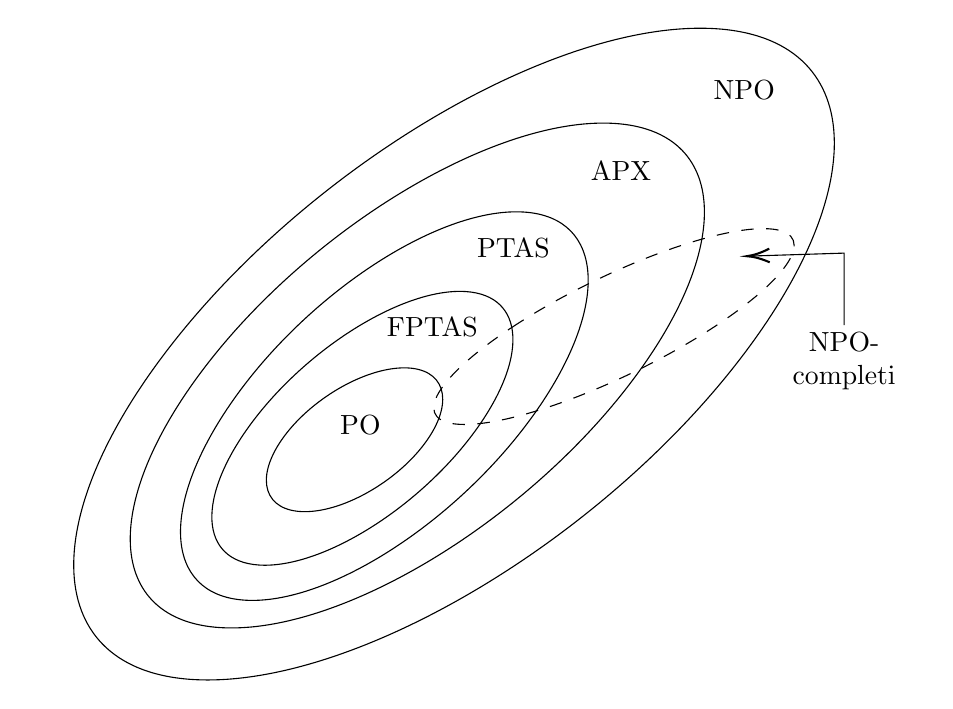
\begin{tikzpicture}[x=0.75pt,y=0.75pt,yscale=-1,xscale=1]
%uncomment if require: \path (0,477); %set diagram left start at 0, and has height of 477

%Shape: Ellipse [id:dp4588658322810296] 
\draw   (310.61,174.5) .. controls (376.13,87.79) and (491.77,17.5) .. (568.88,17.5) .. controls (645.98,17.5) and (655.37,87.79) .. (589.84,174.5) .. controls (524.31,261.21) and (408.68,331.5) .. (331.57,331.5) .. controls (254.46,331.5) and (245.08,261.21) .. (310.61,174.5) -- cycle ;
%Shape: Ellipse [id:dp4441062862246874] 
\draw   (327.15,184.82) .. controls (376.62,117.65) and (463.91,63.2) .. (522.11,63.2) .. controls (580.32,63.2) and (587.41,117.65) .. (537.94,184.82) .. controls (488.48,251.99) and (401.19,306.44) .. (342.98,306.44) .. controls (284.77,306.44) and (277.68,251.99) .. (327.15,184.82) -- cycle ;
%Shape: Ellipse [id:dp42532014972954124] 
\draw   (341.82,199.56) .. controls (376.94,147.86) and (438.92,105.95) .. (480.25,105.95) .. controls (521.58,105.95) and (526.61,147.86) .. (491.49,199.56) .. controls (456.37,251.26) and (394.39,293.17) .. (353.06,293.17) .. controls (311.73,293.17) and (306.7,251.26) .. (341.82,199.56) -- cycle ;
%Shape: Ellipse [id:dp9403889034822421] 
\draw   (350.81,210.25) .. controls (376.75,173.81) and (422.52,144.28) .. (453.04,144.28) .. controls (483.57,144.28) and (487.28,173.81) .. (461.34,210.25) .. controls (435.4,246.68) and (389.63,276.22) .. (359.11,276.22) .. controls (328.58,276.22) and (324.87,246.68) .. (350.81,210.25) -- cycle ;
%Shape: Ellipse [id:dp9056149450292196] 
\draw   (367.2,215.78) .. controls (380.43,196.64) and (406.86,181.13) .. (426.24,181.13) .. controls (445.62,181.13) and (450.6,196.64) .. (437.38,215.78) .. controls (424.15,234.91) and (397.71,250.42) .. (378.34,250.42) .. controls (358.96,250.42) and (353.97,234.91) .. (367.2,215.78) -- cycle ;
%Shape: Ellipse [id:dp18032210948172078] 
\draw  [dash pattern={on 4.5pt off 4.5pt}] (478.73,161.23) .. controls (518.48,135.18) and (572.44,114.06) .. (599.25,114.06) .. controls (626.06,114.06) and (615.57,135.18) .. (575.82,161.23) .. controls (536.07,187.29) and (482.11,208.41) .. (455.3,208.41) .. controls (428.48,208.41) and (438.98,187.29) .. (478.73,161.23) -- cycle ;
%Straight Lines [id:da10034962558485494] 
\draw    (638.18,160.5) -- (638.18,125.85) -- (593.29,127.26) ;
\draw [shift={(591.29,127.33)}, rotate = 358.2] [color={rgb, 255:red, 0; green, 0; blue, 0 }  ][line width=0.75]    (10.93,-3.29) .. controls (6.95,-1.4) and (3.31,-0.3) .. (0,0) .. controls (3.31,0.3) and (6.95,1.4) .. (10.93,3.29)   ;

% Text Node
\draw (574.07,41.64) node [anchor=north west][inner sep=0.75pt]   [align=left] {NPO};
% Text Node
\draw (514.9,80.38) node [anchor=north west][inner sep=0.75pt]   [align=left] {APX};
% Text Node
\draw (460.1,117.56) node [anchor=north west][inner sep=0.75pt]   [align=left] {PTAS};
% Text Node
\draw (416.67,155.6) node [anchor=north west][inner sep=0.75pt]   [align=left] {FPTAS};
% Text Node
\draw (394.14,202.63) node [anchor=north west][inner sep=0.75pt]   [align=left] {PO};
% Text Node
\draw (638.18,178) node   [align=left] {\begin{minipage}[lt]{51.43pt}\setlength\topsep{0pt}
\begin{center}
NPO-completi
\end{center}

\end{minipage}};


\end{tikzpicture}
\caption{Rappresentazione insiemistica delle classi di complessità.}
\label{fig:compsets}
\end{figure}



\section{Terminologia riguardante i problemi}
\subsection{Grafi}
I grafi non orientati sono $G=(V,E)$ (vertici e lati), dove 
$$
E \in {V\choose{2}}
$$
Il \textbf{grado} di un vertice $x$ $d(x)$ è il numero di lati incidenti su 
tale vertice. Il numero di vertici è $n = |V|$, mentre $m = |E|$. 
In un grafo non orientato un \textbf{cammino} di lunghezza $k$ 
$$
\pi = v_1, v_2, \cdots, v_k
$$
tale che $\forall v_{i} \in \pi :\exists \{v_i, v_{i+1}\} \in E$. 
Un cammino senza ripetizioni di vertici è chiamato \textit{semplice}, altrimenti
è definito \textit{non semplice}. Un \textbf{circuito} è un cammino semplice 
chiuso di lunghezza $\geq 3$. La \textbf{connessione} tra due vertici $x$ e $y$
è denotata $x \leadsto y$ e sussiste se esiste un cammino da $x$ a $y$ 
(e, di conseguenza, da $y$ a $x$); 
questa nozione è inoltre una relazione di equivalenza (totale), gode infatti 
di riflessività, transitività e simmetria. Gli insiemi di vertici mutuamente 
connessi formano le \textbf{componenti connesse} di un grafo.
